A brief introduction into nonlinear continuum mechanics and the relevant governing equations will be presented in this section. 

\subsection{Kinematics: motion and deformation}\label{sec:kinematics}



Let $\mathcal{B}_0 \subset \mathbb{R}^3$ denote an open, bounded, and connected set representing the reference (undeformed) configuration of an elastic body. The motion of the body is described by a mapping
\[
\vect{\phi} : \mathcal{B}_0\times \mathbb{R} \rightarrow \mathbb{R}^3,
\]
assumed to be sufficiently smooth, one-to-one, and orientation preserving. For each material point $\vect{X} \in \mathcal{B}_0$, the mapping $\vect{\phi}$ assigns its current position $\vect{x} \in \mathbb{R}^3$ at time $t$ according to
\[
\vect{x} = \vect{\phi}(\vect{X},t),
\qquad
\mathcal{B}(t) = \vect{\phi}(\mathcal{B}_0,t),
\]
see Figure~\ref{fig:superpotato}. The deformation gradient associated with the motion $\vect{\phi}$ is defined as
\[
\vect{F} : \mathcal{B}_0\times \mathbb{R} \rightarrow \mathbb{R}^{3\times 3}, 
\qquad 
\vect{F} = \vect{\nabla}_0 \vect{\phi}(\vect{X},t).
\]

From $\vect{F}$, the cofactor tensor $\vect{H}$ and the Jacobian determinant $J$ are introduced as
\begin{equation}\label{eqn:H and J classical}
	\vect{H} = (\text{det} \vect{F})\,\vect{F}^{-T}
	= \frac{1}{2}\,\vect{F} \Cross \vect{F},
	\qquad
	J = \text{det} \vect{F}
	= \frac{1}{6}\,(\vect{F} \Cross \vect{F}) : \vect{F},
\end{equation}
where the tensor cross product is defined componentwise by
\[
(\vect{A} \Cross \vect{B})_{iI}
= \mathcal{E}_{ijk}\mathcal{E}_{IJK} A_{jJ} B_{kK},
\qquad
\forall\, \vect{A}, \vect{B} \in \mathbb{R}^{3\times 3},
\]
and $\mathcal{E}_{ijk}$ (or $\mathcal{E}_{IJK}$) denotes the components of the third-order alternating tensor\footnote{The use of repeated indices implies summation, unless otherwise stated. In addition, lower case and capital case indices $\{i,j,k\}$ and $\{I,J,K\}$ will be used to represent the deformed and reference configurations, respectively.}.
%

\begin{figure}[htbp]
	\begin{center}
		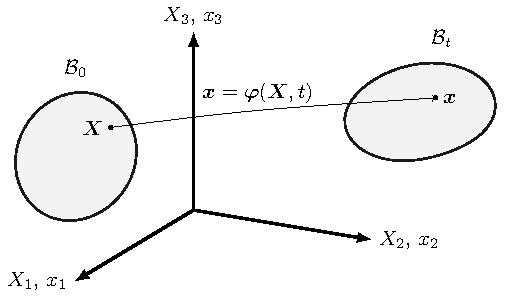
\includegraphics[width=0.6\textwidth]{figures/mapping_continuum.pdf}
	\end{center}
	\caption{The mapping $\vect{\phi}$ and the mechanical and thermal portions of the boundary where Dirichlet conditions are imposed in the reference (and deformed) configurations, namely $\partial_{\vect{\phi}}\mathcal{B}_0$ (and $\partial_{\vect{\phi}}\mathcal{B}$) and $\partial_{\theta}\mathcal{B}_0$ (and $\partial_{{\theta}}\mathcal{B}$).}
	\label{fig:superpotato}
\end{figure}


% \footnote{In addition, throughout the paper, the symbol $(\cdot)$ is used to indicate the scalar product or contraction of a single index $\vect{a}\cdot \vect{b}=a_i b_i$; the symbol $(:)$ is used to indicate double contraction of two indices $\vect{A}:\vect{B}=A_{ij}B_{ij}$; the symbol $(\times)$ is used to indicate the cross product between vectors $[\vect{a} \times \vect{b}]_i=\mathcal{E}_{ijk}a_jb_k$ and the symbol $(\otimes)$ is used to indicate the outer or dyadic product $[\vect{a}\otimes \vect{b}]_{ij}=a_ib_j$.}. 
%As shown in References \cite{Bonet_cross_product_2016,Bonet_polyconvexity_2015}, the definitions of $\vect{H}$ and $J$ in \eqref{eqn:H and J tensor cross product expression}, although equivalent to those in \eqref{eqn:H and J classical}, are very appealing as they yield simpler expressions for their directional derivatives \cite{Bonet_polyconvexity_2015,Bonet_cross_product_2016, Gil_electro_partI_2016,Gil_electro_partII_2016,Gil_electro_partIII_2016, Betsch_EM_thermo_2017}. 






\subsection{Governing equations in non-linear thermo-electro-mechanics: conservation of linear momentum and angular momentum}\label{sec:conservation of linear momentum}

The local form of the conservation of linear momentum \cite{Gonzalez_book} can be written as
%
\begin{equation}\label{eqn:local form conservation of linear momentum}
\begin{aligned}
  \rho_0\dot{\vect{v}} - \div\vect{P} - \vect{f}_0& = \vect{0};&\qquad &\text{in}\,\,\B_0\times \left[0,T\right];\\
  %
  \P\cdot\vect{N}& = \vect{t}_0;&\qquad&\text{on}\,\,\partial_{\boldsymbol{t}}\B_0\times \left[0,T\right];\\
  %
  \vect{\phi} &= \bar{\vect{\phi}};&\qquad & \text{on}\,\,\partial_{\vect{\phi}}\B_0\times \left[0,T\right];\\
  %
  \left.\dot{\vect{\phi}}\right|_{t=0}&=\dot{\bar{\vect{\phi}}};&\qquad &\text{in}\,\,\B_0;\\
  %#
  \left.\vect{\phi}\right|_{t=0}&=\bar{\vect{\phi}};&\qquad
  &\text{in}\,\,\B_0,
\end{aligned}
\end{equation}
%
where $\rho_0: \mathcal{B}_0\rightarrow \mathbb{R}^{+}$ represents the mass density of the continuum in the reference configuration, $\vect{v}$ the velocity field and 
 $\left(\dot{\bullet}\right):=\frac{d (\bullet)}{dt}$ denotes differentiation with respect to time. 
Furthermore, $\vect{f}_0$ represents a body force per unit undeformed volume $\mathcal{B}_0$ and $\vect{t}_0$, the traction force per unit undeformed area applied on $\partial_{\boldsymbol{t}}\mathcal{B}_0\subset \partial \mathcal{B}_0$, such that $\partial_{\boldsymbol{t}}\mathcal{B}_0 \cup \partial_{\vect{\phi}}\mathcal{B}_0 = \partial\mathcal{B}_0$ and $\partial_{\boldsymbol{t}}\mathcal{B}_0 \cap \partial_{\vect{\phi}}\mathcal{B}_0 = \emptyset$. 
Finally,  $\vect{P}$ %\footnote{Notice that in previous publications \cite{Gil_electro_partI_2016,Gil_electro_partII_2016,Gil_electro_partIII_2016} the authors have pursued a formulation in terms of the first Piola-Kirchhoff stress tensor $\vect{P}$, related to the second Piola-Kirchhoff stress tensor as $\vect{P} = \vect{FS}$. 
%In this paper, the design of an energy-momentum time integrator scheme, and in particular, the satisfaction of conservation of angular momentum, motivates the use of the symmetric stress tensor $\vect{S}$.} 
represents the first Piola-Kirchhoff stress tensor and the local conservation of angular momentum leads to the well-known tensor condition $\vect{PF}^T = \vect{FP}^T$. Finally, $T$ represents the upper bound for the time variable $t\in\left[0,T\right]$.
%


\subsection{Governing equations in non-linear thermo-electro-mechanics: Gauss's and Faraday's laws}\label{sec:Gauss and Faraday}


In the electrostatics case considered, the local form of the Gauss’s law can be written in a Lagrangian setting as
%
\begin{equation}\label{eqn:Gauss law}
\begin{aligned}
\div\vect{D}_0 - \rho_0^e&=0;&\qquad &\text{in}\,\mathcal{B}_0\times \left[0,T\right]\\
%
%
\vect{D}_0\cdot\vect{N}& = -\omega_0^e;&\qquad &\text{on}\, \partial_{\omega}\mathcal{B}_0\times \left[0,T\right].
%
%
\end{aligned}
\end{equation}
%
where $\vect{D}_0$ is the Lagrangian electric displacement vector, $\rho_{0}^e$ represents an electric volume charge per unit of undeformed volume $\mathcal{B}_0$ and $\omega_0^e$, the electric surface charge per unit of undeformed area $\partial_{\omega}\mathcal{B}_0\in\partial\mathcal{B}_0$. %Alternatively, the spatial electric displacement vector $\vect{D}$ can be obtained through the area push forward relationship $\vect{D}_0=\vect{H}^T\vect{D}$.
Furthermore, the Faraday’s law can be written in a Lagrangian setting as
%
\begin{equation}\label{eqn:Faraday}
\begin{aligned}
\vect{E}_0 &= -\vect{\nabla}_{0}\varphi;&\qquad
&\text{in}\,\mathcal{B}_0\times \left[0,T\right];\\
%
\varphi&=\bar{\varphi};&\qquad &\text{on}\,\partial_{\varphi}\mathcal{B}_0\times \left[0,T\right],
%
\end{aligned}
\end{equation}
%
where $\vect{E}_0$ is the Lagrangian electric field vector and $\varphi$, the scalar electric potential. In \eqref{eqn:Faraday}, $\partial_{\varphi}\mathcal{B}_0\subset\partial\mathcal{B}_0$ represents the part of
the boundary where essential electric potential boundary conditions are applied such that $\partial_{\omega}\mathcal{B}_0\cup \partial_{\varphi}\mathcal{B}_0=\partial\mathcal{B}_0$ and $\partial_{\omega}\mathcal{B}_0\cap \partial_{\varphi}\mathcal{B}_0=\emptyset$. 



\subsection{Governing equations in non-linear thermo-electro-mechanics: conservation of energy and Fourier's law}\label{sec:conservation of energy}

\Blue{Miguel: del mismo modo que antes hemos introducido la ley de Faraday junto con las ecuaciones de conservación de Gauss, aquí debemos incluir la ley de Fourier con la conservación de energía. La excepción se encuentra en la conservación del momento, donde la ley constitutiva merece una sección a parte.}

The balance of energy equation can be written as
%
\begin{equation}\label{eqn:local form energy}
\begin{aligned}
\theta\dot{\eta}  - \mathcal{D} + \div\vect{Q} - R_{\theta} & = 0;&\qquad& \text{in}\,\,\mathcal{B}_0\times \left[0,T\right];\\
%
\vect{Q}\cdot\vect{N}& = -Q_{\theta};&\qquad&\text{on}\,\, \partial_{Q}\mathcal{B}_0\times \left[0,T\right];\\
%
\theta & = \bar{\theta};&\qquad&\text{on}\,\,\partial_{\theta}\mathcal{B}_0\times \left[0,T\right];\\
%%#
\left.{\theta}\right|_{t=0}&={\bar{\theta}};&\qquad& \text{in}\,\,\mathcal{B}_0,
\end{aligned}
\end{equation}
%
where $\theta$ is the absolute temperature field and $\eta$ and $\vect{Q}$, the entropy and heat flux per unit undeformed volume $\mathcal{B}_0$, respectively. In addition, $R_{\theta}$  represents the heat source per unit undeformed volume $\mathcal{B}_0$ and $Q_{\theta}$, the heat source per unit undeformed area applied on $\partial_{Q}\mathcal{B}_0\subset\partial\mathcal{B}_0$. In \eqref{eqn:local form energy}, $\partial_{\theta}\mathcal{B}_0$ represents the part of the boundary $\partial\mathcal{B}_0$ where essential temperature boundary conditions are applied such that $\partial_{Q}\mathcal{B}_0\cup\partial_{\theta}\mathcal{B}_0 = \partial\mathcal{B}_0$ and $\partial_{Q}\mathcal{B}_0\cap\partial_{\theta}\mathcal{B}_0 = \emptyset$. Furthermore, $\mathcal{D}$ correspond with the dissipation inequality. 


With the aim of simplifying the time discretisation of \eqref{eqn:local form energy}, the authors in \Red{XXXX} proposed an alternative but equivalent re-expression (at the continuum level) to that in \eqref{eqn:local form energy} as
%
\begin{equation}\label{eqn:local form energy our format}
\begin{aligned}
\frac{d}{dt}\left(\theta\eta\right) - \dot{\theta}\eta -\mathcal{D} + \div\vect{Q} - R_{\theta} & = 0;&\qquad& \text{in}\,\,\mathcal{B}_0\times \left[0,T\right];\\
%
\vect{Q}\cdot\vect{N}& = -Q_{\theta};&\qquad&\text{on}\,\, \partial_{Q}\mathcal{B}_0\times \left[0,T\right];\\
%
\theta & = \bar{\theta};&\qquad&\text{on}\,\,\partial_{\theta}\mathcal{B}_0\times \left[0,T\right];\\
%
%#
\left.{\theta}\right|_{t=0}&={\bar{\theta}};&\qquad& \text{in}\,\,\mathcal{B}_0.
%
\end{aligned}
\end{equation}

In this work we will advocate for \eqref{eqn:local form energy our format} instead of \eqref{eqn:local form energy}.

The Fourier law relates the spatial heat flux $\vect{q}$ and the spatial gradient of $\theta$ by virtue of the following expression
%
\begin{equation}
  \label{eqn:Duhamel}
  \vect{q} = -\vect{k}\vect{\nabla}\theta,
\end{equation}
%
where $\vect{k}$ represents the semi-positive definite second order thermal conductivity tensor in the deformed configuration and $\vect{\nabla}(\bullet)$ the spatial gradient operator. As customary in continuum mechanics, the relation between $\vect{q}$ and its material counterpart $\vect{Q}$ featuring in equation \eqref{eqn:local form energy our format} can be carried out by making use of the Gauss' theorem and the Nanson's rule (i.e. $d\vect{a}=\vect{H}d\vect{A}$) as 
%
\begin{equation}
  \label{eqn:flux}
  \int_{\mathcal{B}}\div\vect{q}\,dv = 
    \int_{\partial\mathcal{B}}\vect{q}\cdot\,d\vect{a} =
    \int_{\partial\mathcal{B}_0}\vect{Q}\cdot\,d\vect{A},
\end{equation}
%
%Application of the Gauss's theorem on both sides of \eqref{eqn:flux} leads to
%%
%\begin{equation}
%\int_{\partial\mathcal{B}}\vect{q}\cdot d\vect{a} = \int_{\partial\mathcal{B}_0}\vect{Q}\cdot d\vect{A}. 
%\end{equation}
%
%Making use of the Nanson's rule (i.e. $d\vect{a} = \vect{H}d\vect{A}$) and considering \eqref{eqn:Duhamel}, it is possible to express $\vect{Q}$ as
%
where $\div(\bullet)$ represents the spatial divergence operator and with 
%
\begin{equation}
  \label{eqn: Q I}
  \vect{Q} = \vect{H}^T\vect{q} = -\vect{H}^T\vect{k}\vect{\nabla}\theta.
\end{equation}

The spatial gradient of $\theta$ \eqref{eqn: Q I} can be conveniently related to its material counterpart as
%
\begin{equation}
  \label{eqn:spatial gradient of theta}
  \vect{\nabla}\theta = \vect{F}^{-T}\vect{\nabla}\theta = J^{-1}\vect{H}\vect{\nabla}\theta.
\end{equation}

Finally, introduction of \eqref{eqn:spatial gradient of theta} into \eqref{eqn: Q I} yields 
%
\begin{equation}
  \vect{Q} = -\vect{K}\vect{\nabla}\theta;\qquad
  \vect{K} = J^{-1}\vect{H}^T\vect{k}\vect{H}.
\end{equation}



